\chapter{Análisis y comparativa de paquetes}
\label{cha:analisis y comparativa de paquetes}

Tras la exposición de las diferentes variables y métricas que conformaran la evaluación, se realiza el
correspondiente análisis y comparación de paquetes. Inicialmente, el análisis será individual de cada
paquete, señalando aspectos relativos a otros paquetes si fuese necesario. En la segunda sección, se 
realizará una comparación conjunta de todos los paquetes analizados.

\section{Evaluación individual de paquetes}
\label{sec:evaluacion individual de paquetes}

Tal y como se ha especificado en la introducción, se procede con el análisis individual de cada paquete.
A lo largo de la misma, se introducirán aspectos relativos a ciertos paquetes, como el tipo de analizador
y los resultados obtenidos empleando distintos tipos de herramientas. Para cada paquete se especificará 
una tabla de resultados y una imagen de los mismos resultados dispuestos gráficamente.

\section*{inscriptis}

El primer paquete sometido a análisis será \textbf{inscriptis}, el cual debemos instalar e importar en el
fragmento de código respectivo. En cuanto a su instalación, es muy sencilla, simplemente se debe ejecutar
la siguiente instrucción en la línea de comandos: \emph{\$ pip install inscriptis}.

\begin{codefloat}
    \inputencoding{latin1}
    \lstinputlisting[style=CppExample, showstringspaces=false]{scripts/script-inscriptis.py}
    \inputencoding{utf8}
    \caption{Función de ejecución de inscriptis}
    \label{cod:funcion de ejecucion de inscriptis}
\end{codefloat}

En cuanto al código mostrado en \ref{cod:funcion de ejecucion de inscriptis}, es muy simple. Se itera sobre 
los archivos HTML a analizar, y se emplea la función \emph{get\_text()} para obtener la información deseada. 
Dicha información se almacena posteriormente de forma ordenada sobre un diccionario.

Para conservar la información obtenida y no ejecutar el algoritmo múltiples veces, el diccionario obtenido
se almacena en un archivo \emph{json} propio del paquete. De esta forma, el archivo \emph{inscriptis.json} 
conserva todos los fragmentos de texto obtenidos del minado web anterior. Este mismo procedimiento se 
realiza para el resto de paquetes.

Una vez ejecutado el algoritmo, se realizan todos los cálculos pertinentes y se determinan las puntuaciones
obtenidas. En el caso de \textbf{inscriptis}, se muestran en la tabla
\ref{tab:tabla - resultados de la evaluacion de inscriptis} los resultados obtenidos.

\begin{table}[h]
    \begin{center}
      \begin{tabular}{| c | c | c | c | c | c | c | c |} \hline 
       \textbf{Nombre} & \textbf{Accuracy} & \textbf{Precision}  & \textbf{Recall} & \textbf{F1} & \textbf{RAM(\%)} & \textbf{CPU(\%)} & \textbf{Time Exec.(s)} \\ \hline
       inscriptis & 0.5414 & 0.5404 & 0.9875 & 0.6985 & 45.0 & 0.2 & 2.1005 \\ \hline
      \end{tabular}
      \caption{Tabla - Resultados de la evaluación de inscriptis}
      \label{tab:tabla - resultados de la evaluacion de inscriptis}
    \end{center}
\end{table} 

En forma de gráfica, se muestra en la figura \ref{img:grafica - resultados de la evaluacion de inscriptis}
los cálculos obtenidos en referencia a las métricas independientes del entorno de ejecución. Analizando
estas métricas, y sabiendo que \emph{f1} determina la calidad en general de la extracción, podemos concluir
que \textbf{inscriptis} realiza un equilibrado trabajo en el minado web.

\begin{figure}[tphb]
    \centering
    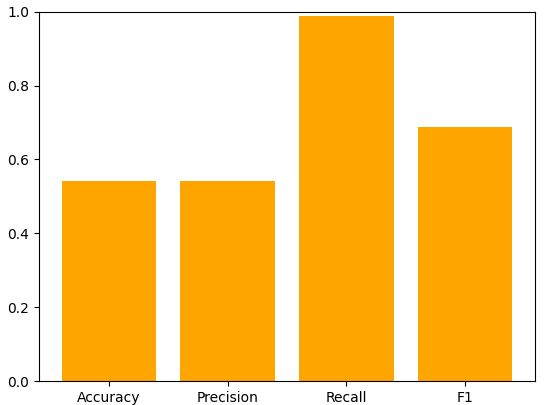
\includegraphics[width=5in]{resultados-inscriptis.jpg}
    \caption{Gráfica - Resultados de la evaluación de inscriptis}
    \label{img:grafica - resultados de la evaluacion de inscriptis}
\end{figure}

Por otro lado, respecto a las métricas dependientes del entorno, al solo tener una medición de referencia 
no podemos decir demasiado. El uso de memoria RAM parece elevado dadas las especificaciones del entorno. 
Por el contrario, el uso de CPU es mínimo. Algo sorprendente es que \textbf{inscriptis} haya sido capaz de 
analizar 101 documentos HTML en únicamente dos segundos.

\section*{Beautiful Soup}

El segundo paquete sometido a análisis será \textbf{Beautiful Soup}, el cual debemos instalar e importar 
en el fragmento de código respectivo. En cuanto a su instalación, simplemente se debe ejecutar la siguiente 
instrucción en la línea de comandos: \emph{\$ pip install beautifulsoup4}.

Como se observa en el fragmento de código \ref{cod:funcion de ejecucion beautiful soup}, la función es muy
similar a la vista con \textbf{inscriptis}. Se itera sobre los documentos HTML a analizar y se aplica la
función \emph{get\_text()} para extraer la información.

\begin{codefloat}
    \inputencoding{latin1}
    \lstinputlisting[style=CppExample, showstringspaces=false]{scripts/script-beautifulsoup.py}
    \inputencoding{utf8}
    \caption{Función de ejecución de Beautiful Soup}
    \label{cod:funcion de ejecucion beautiful soup}
\end{codefloat}

Debemos recordar que \textbf{Beautiful Soup} permite seleccionar entre varios tipos de analizadores, ya sea
\emph{html.parse}, \emph{lxml} o \emph{html5lib}. Tras la ejecución de \textbf{Beautiful Soup} empleando
\emph{html.parse} como analizador, se procede con el cálculo de métricas. Los resultados obtenidos se 
muestran en la tabla \ref{tab:tabla - resultados de la evaluacion de beautiful soup html.parse}.

\begin{table}[h]
    \begin{center}
      \begin{tabular}{| c | c | c | c | c | c | c | c |} \hline 
       \textbf{Nombre} & \textbf{Accuracy} & \textbf{Precision}  & \textbf{Recall} & \textbf{F1} & \textbf{RAM(\%)} & \textbf{CPU(\%)} & \textbf{Time Exec.(s)} \\ \hline
       Beau. Soup & 0.5165 & 0.5129 & 0.9928 & 0.6764 & 47.0 & 4.3 & 4.0882 \\ \hline
      \end{tabular}
      \caption{Tabla - Resultados de la evaluación de Beautiful Soup \emph{(html.parse)}}
      \label{tab:tabla - resultados de la evaluacion de beautiful soup html.parse}
    \end{center}
\end{table} 

Se emplea ahora \emph{lxml} como analizador estándar y se procede con el cálculo de métricas. Los resultados
obtenidos se muestran en la tabla \ref{tab:tabla - resultados de la evaluacion de beautiful soup lxml}.

\begin{table}[h]
    \begin{center}
      \begin{tabular}{| c | c | c | c | c | c | c | c |} \hline 
       \textbf{Nombre} & \textbf{Accuracy} & \textbf{Precision}  & \textbf{Recall} & \textbf{F1} & \textbf{RAM(\%)} & \textbf{CPU(\%)} & \textbf{Time Exec.(s)} \\ \hline
       Beau. Soup & 0.5165 & 0.5129 & 0.9928 & 0.6764 & 38.1 & 3.4 & 3.2183 \\ \hline
      \end{tabular}
      \caption{Tabla - Resultados de la evaluación de Beautiful Soup \emph{(lxml)}}
      \label{tab:tabla - resultados de la evaluacion de beautiful soup lxml}
    \end{center}
\end{table}

Se emplea ahora \emph{html5lib} como analizador estándar y se procede con el cálculo de métricas. Los 
resultados obtenidos se muestran en la tabla 
\ref{tab:tabla - resultados de la evaluacion de beautiful soup html5lib}.

\begin{table}[h]
    \begin{center}
      \begin{tabular}{| c | c | c | c | c | c | c | c |} \hline 
       \textbf{Nombre} & \textbf{Accuracy} & \textbf{Precision}  & \textbf{Recall} & \textbf{F1} & \textbf{RAM(\%)} & \textbf{CPU(\%)} & \textbf{Time Exec.(s)} \\ \hline
       Beau. Soup & 0.1327 & 0.1315 & 0.9921 & 0.2323 & 39.1 & 3.4 & 9.8604 \\ \hline
      \end{tabular}
      \caption{Tabla - Resultados de la evaluación de Beautiful Soup \emph{(html5lib)}}
      \label{tab:tabla - resultados de la evaluacion de beautiful soup html5lib}
    \end{center}
\end{table}

En forma de gráfica, se muestra en \ref{img:grafica - resultados de la evaluacion de beautiful soup} los 
cálculos obtenidos en referencia a las métricas independientes del entorno de ejecución. Realizando un
análisis, podemos determinar que el uso de \emph{html.parse} o \emph{lxml} no altera la calidad de la 
información obtenida. Por el contrario cuando se emplea \emph{html5lib} tanto la cantidad de predicciones 
correctas, como la exclusión de contenido \emph{boilerplate} se reduce drásticamente.

\begin{figure}[tphb]
    \centering
    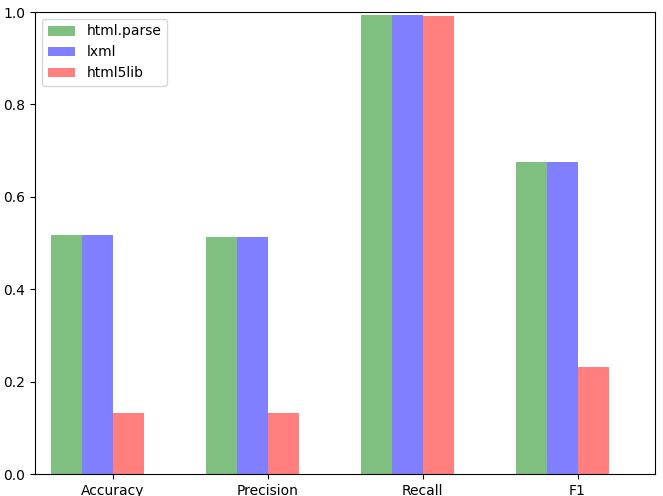
\includegraphics[width=4.6in]{resultados-beautifulsoup.jpg}
    \caption{Gráfica - Resultados de la evaluación de Beautiful Soup}
    \label{img:grafica - resultados de la evaluacion de beautiful soup}
\end{figure}

Por otro lado, respecto a las métricas dependientes del entorno, el uso de memoria RAM, al igual que el uso
de CPU, es similar en todos los analizadores. Véase \ref{img:grafica - resultados de la evaluacion de beautiful soup 2}.

\begin{figure}[tphb]
    \centering
    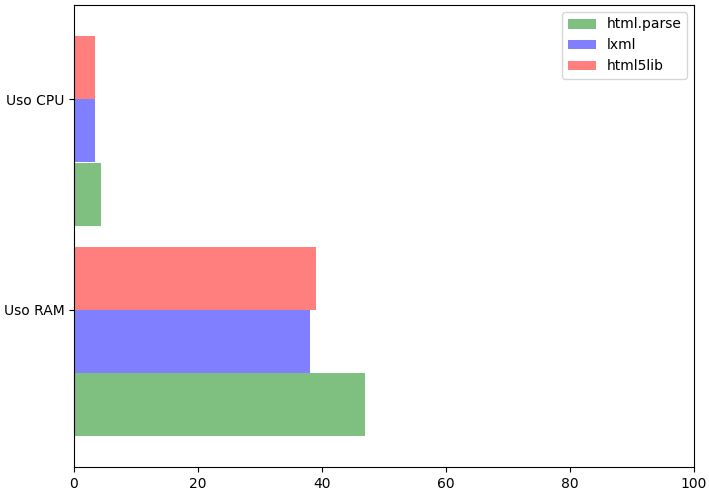
\includegraphics[width=4.6in]{resultados-beautifulsoup2.jpg}
    \caption{Gráfica - Resultados de la evaluación de Beautiful Soup 2}
    \label{img:grafica - resultados de la evaluacion de beautiful soup 2}
\end{figure}

\section*{jusText}

Continuamos con el análisis de \textbf{jusText}, el cual debemos instalar e importar en el fragmento de 
código respectivo. En cuanto a su instalación, simplemente se debe ejecutar la siguiente instrucción en la 
línea de comandos: \emph{\$ pip install justext}.

Como se observa en el fragmento de código \ref{cod:funcion de ejecucion de jusText}, la forma en la que
se extrae texto de documentos HTML es muy similar a las vistas anteriormente. La principal diferencia es
que en este caso \textbf{jusText}, previamente a la extracción, realiza las siguientes acciones:

\begin{itemize}
    \item Clasificación de bloques.
    \item Preprocesamiento de bloques de cabecera.
    \item Reclasificación de bloques.
    \item Postprocesamiento de bloques de cabecera.
\end{itemize}

\begin{codefloat}
    \inputencoding{latin1}
    \lstinputlisting[style=CppExample, showstringspaces=false]{scripts/script-justext.py}
    \inputencoding{utf8}
    \caption{Función de ejecución de jusText}
    \label{cod:funcion de ejecucion de jusText}
\end{codefloat}

Como el resto de algoritmos, para conservar la información obtenida y no ejecutar el código múltiples 
veces, el diccionario obtenido se almacena en un archivo \emph{json} propio del paquete. De esta forma, 
el \emph{justext.json} conserva todos los fragmentos de texto obtenidos del minado web anterior.

Una vez ejecutado el algoritmo, se realizan todos los cálculos pertinentes y se determinan las puntuaciones 
obtenidas. En el caso de \textbf{jusText}, los resultados obtenidos se muestran en la tabla 
\ref{tab:tabla - resultados de la evaluacion de justext}.

\begin{table}[h]
    \begin{center}
      \begin{tabular}{| c | c | c | c | c | c | c | c |} \hline 
       \textbf{Nombre} & \textbf{Accuracy} & \textbf{Precision}  & \textbf{Recall} & \textbf{F1} & \textbf{RAM(\%)} & \textbf{CPU(\%)} & \textbf{Time Exec.(s)} \\ \hline
       jusText & 0.7668 & 0.8649 & 0.8573 & 0.8610 & 45.1 & 0.5 & 2.9546 \\ \hline
      \end{tabular}
      \caption{Tabla - Resultados de la evaluación de jusText}
      \label{tab:tabla - resultados de la evaluacion de justext}
    \end{center}
\end{table}

En forma de gráfica, se muestra en la figura \ref{img:grafica - resultados de la evaluacion de justext}
los cálculos obtenidos en referencia a las métricas independientes del entorno de ejecución. Con un simple
vistazo, es posible determinar que el algoritmo de \textbf{jusText} realiza un buen trabajo en al selección
de contenido relevante. 

\begin{figure}[tphb]
    \centering
    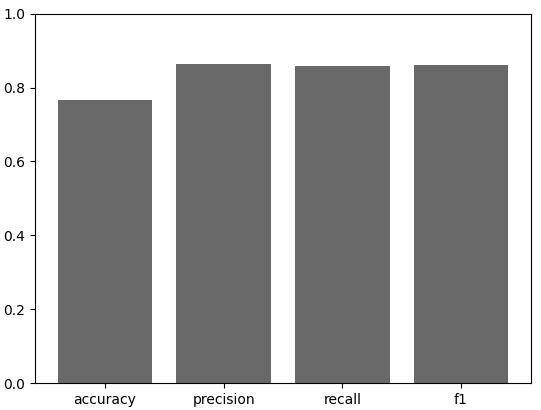
\includegraphics[width=5in]{resultados-justext.jpg}
    \caption{Gráfica - Resultados de la evaluación de jusText}
    \label{img:grafica - resultados de la evaluacion de justext}
\end{figure}

Por otro lado, con respecto a las métricas dependientes del entorno de ejecución, se debe remarcar que
\textbf{jusText} es un paquete de minado web muy bien optimizado. A pesar de realizar todo el trabajo previo
a la extracción, mantiene un buen tiempo de ejecución y escaso uso de la CPU.

\section*{html\_text}

El siguiente paquete sometido a análisis será \textbf{html\_text}, el cual debemos instalar e importar en 
el fragmento de código respectivo. En cuanto a su instalación, simplemente se debe ejecutar la siguiente 
instrucción en la línea de comandos: \emph{\$ pip install html-text}.

\begin{codefloat}
    \inputencoding{latin1}
    \lstinputlisting[style=CppExample, showstringspaces=false]{scripts/script-htmltext.py}
    \inputencoding{utf8}
    \caption{Función de ejecución de html\_text}
    \label{cod:funcion de ejecucion de htmltext}
\end{codefloat}

En el fragmento de código \ref{cod:funcion de ejecucion de htmltext} se muestra como \textbf{html\_text} 
extrae texto de los diferentes documentos HTML. La función \emph{extract\_text()} emplea expresiones 
\emph{xPath} y normalizaciones de espacio para obtener una mejor calidad en los resultados.

Una vez ejecutado el algoritmo, se realizan todos los cálculos pertinentes y se determinan las puntuaciones 
obtenidas. En el caso de \textbf{html\_text}, los resultados obtenidos se muestran en la tabla 
\ref{tab:tabla - resultados de la evaluacion de htmltext}.

\begin{table}[h]
    \begin{center}
      \begin{tabular}{| c | c | c | c | c | c | c | c |} \hline 
       \textbf{Nombre} & \textbf{Accuracy} & \textbf{Precision}  & \textbf{Recall} & \textbf{F1} & \textbf{RAM(\%)} & \textbf{CPU(\%)} & \textbf{Time Exec.(s)} \\ \hline
       html\_text & 0.5166 & 0.5130 & 0.9928 & 0.6765 & 44.9 & 0.5 & 1.1800 \\ \hline
      \end{tabular}
      \caption{Tabla - Resultados de la evaluación de html\_text}
      \label{tab:tabla - resultados de la evaluacion de htmltext}
    \end{center}
\end{table}

Tanto en la tabla \ref{tab:tabla - resultados de la evaluacion de htmltext} como en su correspondiente
gráfica \ref{img:grafica - resultados de la evaluacion de htmltext}, podemos observar que el algoritmo
cumple asequiblemente con unos requisitos mínimos con respecto a aquellas métricas no dependientes del
entorno de ejecución.

\begin{figure}[tphb]
    \centering
    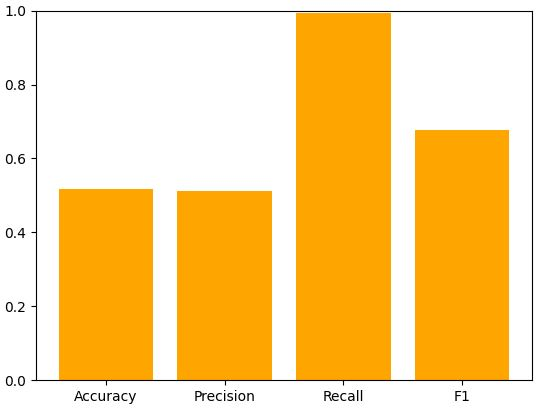
\includegraphics[width=5in]{resultados-htmltext.jpg}
    \caption{Gráfica - Resultados de la evaluación de html\_text}
    \label{img:grafica - resultados de la evaluacion de htmltext}
\end{figure}

En cuanto a las métricas dependientes de entorno, es cierto que el algoritmo emplea pocos recursos, y su
tiempo de ejecución es reducido. Esto se debe a que su heurística es simple, el uso único de expresiones
\emph{xPath} optimiza los recursos. ¿Compensa sobre la calidad de la extracción? Lo veremos en al siguiente
sección, cuando comparemos la \emph{performance} de todos los paquetes.

\section*{html2text}

Otro de los paquetes sometidos a análisis será \textbf{html2text}, el cual debemos instalar e importar en 
el fragmento de código respectivo. En cuanto a su instalación, simplemente se debe ejecutar la siguiente 
instrucción en la línea de comandos: \emph{\$ pip install html2text}.

\begin{codefloat}
    \inputencoding{latin1}
    \lstinputlisting[style=CppExample, showstringspaces=false]{scripts/script-html2text.py}
    \inputencoding{utf8}
    \caption{Función de ejecución de html2text}
    \label{cod:funcion de ejecucion de html2text}
\end{codefloat}

En el fragmento de código \ref{cod:funcion de ejecucion de html2text} se muestra como \textbf{html2text}
extrae texto de los diferentes documentos HTML. Si recordamos, \textbf{html2text} no se caracteriza por
disponer de una heurística compleja, el algoritmo simplemente hace uso de \emph{html.parse} para analizar
el documento y envolver todos los párrafos del texto proporcionado.

\begin{table}[h]
    \begin{center}
      \begin{tabular}{| c | c | c | c | c | c | c | c |} \hline 
       \textbf{Nombre} & \textbf{Accuracy} & \textbf{Precision}  & \textbf{Recall} & \textbf{F1} & \textbf{RAM(\%)} & \textbf{CPU(\%)} & \textbf{Time Exec.(s)} \\ \hline
       html2text & 0.5105 & 0.5107 & 0.9804 & 0.6715 & 44.6 & 1.8 & 4.4020 \\ \hline
      \end{tabular}
      \caption{Tabla - Resultados de la evaluación de html2text}
      \label{tab:tabla - resultados de la evaluacion de html2text}
    \end{center}
\end{table}

Los resultados mostrados, tanto en la tabla \ref{tab:tabla - resultados de la evaluacion de html2text} como
en la gráfica \ref{img:grafica - resultados de la evaluacion de html2text}, hacen reflejo de la simplicidad
de su heurística. A pesar de todo ello, la calidad en general de la extracción no está muy lejos de la media.

\begin{figure}[tphb]
    \centering
    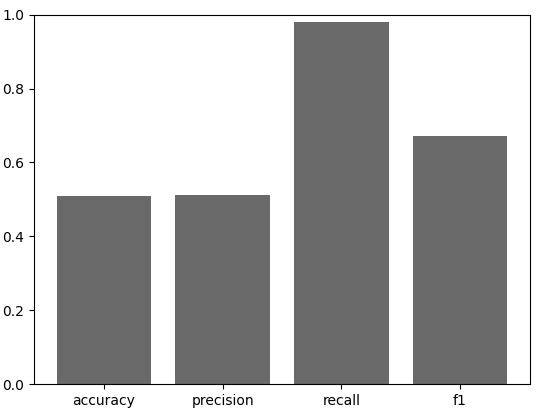
\includegraphics[width=4.7in]{resultados-html2text.jpg}
    \caption{Gráfica - Resultados de la evaluación de html2text}
    \label{img:grafica - resultados de la evaluacion de html2text}
\end{figure}

\section*{Readability}

El siguiente paquete sometido a análisis será \textbf{Readability}, el cual debemos instalar e importar 
en el fragmento de código respectivo. En cuanto a su instalación, simplemente se debe ejecutar la siguiente 
instrucción en la línea de comandos: \emph{\$ pip install readability-lxml}.

\begin{codefloat}
    \inputencoding{latin1}
    \lstinputlisting[style=CppExample, showstringspaces=false]{scripts/script-readability.py}
    \inputencoding{utf8}
    \caption{Función de ejecución de Readability}
    \label{cod:funcion de ejecucion de readability}
\end{codefloat}

En el fragmento de código \ref{cod:funcion de ejecucion de readability} se muestra como \textbf{Readability}
extrae texto de los diferentes documentos HTML. El algoritmo es muy simple y similar a los algoritmos de
otros paquetes. Veamos los resultados de las métricas calculadas.

\begin{table}[h]
    \begin{center}
      \begin{tabular}{| c | c | c | c | c | c | c | c |} \hline 
       \textbf{Nombre} & \textbf{Accuracy} & \textbf{Precision}  & \textbf{Recall} & \textbf{F1} & \textbf{RAM(\%)} & \textbf{CPU(\%)} & \textbf{Time Exec.(s)} \\ \hline
       Readability & 0.8880 & 0.9101 & 0.9370 & 0.9233 & 45.3 & 1.6 & 3.5952 \\ \hline
      \end{tabular}
      \caption{Tabla - Resultados de la evaluación de Readability}
      \label{tab:tabla - resultados de la evaluacion de readability}
    \end{center}
\end{table}

Por otro lado, si recordamos la heurística del paquete, este empleaba la selección del nodo candidato para
encontrar nodos de valor. Tras una primera selección se buscaban nodos adyacentes con el mismo propósito.
Se puede observar tanto en la tabla \ref{tab:tabla - resultados de la evaluacion de readability} como en
la gráfica \ref{img:grafica - resultados de la evaluacion de readability}, que la heurística parece funcionar.
El algoritmo presenta una buena calidad en la extracción, los cálculos de \emph{accuracy} y \emph{precision}
son muy buenos con respecto a los paquetes ya evaluados.

Además de \textbf{Readability}, \textbf{Goose3} empleaba la misma técnica de nodo candidato para encontrar
nodos de valor. Se muestra en la tabla \ref{tab:tabla - comparacion de resultados entre readability y goose3} 
una pequeña comparación entre ambos paquetes, donde los resultados referentes a la calidad de la extracción, 
son muy parejos.

\begin{table}[h]
    \begin{center}
      \begin{tabular}{| c | c | c | c | c | c | c | c |} \hline 
       \textbf{Nombre} & \textbf{Accuracy} & \textbf{Precision}  & \textbf{Recall} & \textbf{F1} & \textbf{RAM(\%)} & \textbf{CPU(\%)} & \textbf{Time Exec.(s)} \\ \hline
       Readability & 0.8880 & 0.9101 & 0.9370 & 0.9233 & 45.3 & 1.6 & 3.5952 \\ \hline
       Goose3 & 0.8658 & 0.9273 & 0.8913 & 0.9089 & 32.2 & 6.1 & 25.9731 \\ \hline
      \end{tabular}
      \caption{Tabla - Comparación de resultados entre Readability \& Goose3}
      \label{tab:tabla - comparacion de resultados entre readability y goose3}
    \end{center}
\end{table}

Además de la comparación vista, más adelante se realizará una evaluación individual de \textbf{Goose3} el
cual hasta entonces, al igual que \textbf{Readability}, parece un algoritmo bastante completo.

\begin{figure}[tphb]
    \centering
    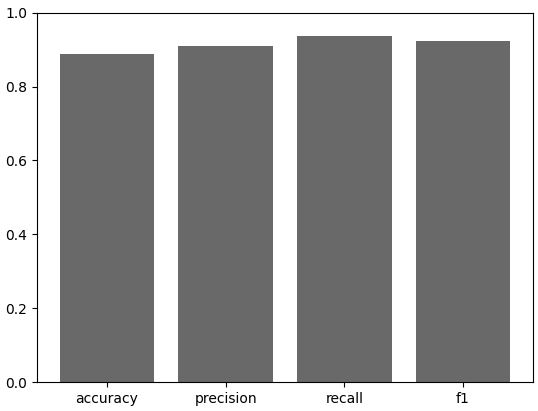
\includegraphics[width=5in]{resultados-readability.jpg}
    \caption{Gráfica - Resultados de la evaluación de Readability}
    \label{img:grafica - resultados de la evaluacion de readability}
\end{figure}

En cuanto a las métricas dependientes del entorno, tanto los resultados de uso de memoria RAM, como el uso
de CPU y el tiempo de ejecución del algoritmo entran dentro de lo estándar. La calidad de la información
extraída y los resultados obtenidos en tiempo de ejecución y empleo de recursos, reflejan una muy buena
optimización del paquete.

\section*{Trafilatura}

Otro paquete sometido a análisis será \textbf{Trafilatura}, el cual debemos instalar e importar 
en el fragmento de código respectivo. En cuanto a su instalación, simplemente se debe ejecutar la siguiente 
instrucción en la línea de comandos: \emph{\$ pip install trafilatura}.

\begin{codefloat}
    \inputencoding{latin1}
    \lstinputlisting[style=CppExample, showstringspaces=false]{scripts/script-trafilatura.py}
    \inputencoding{utf8}
    \caption{Función de ejecución de Trafilatura}
    \label{cod:funcion de ejecucion de trafilatura}
\end{codefloat}

En cuanto a la función de extracción, debemos recordar que \textbf{Trafilatura} dispone de diferentes
configuraciones con las que poder determinar la forma en la que se va a realizar el minado. En el fragmento
de código \ref{cod:funcion de ejecucion de trafilatura} se muestra la función más genérica.

Tanto en la tabla \ref{tab:tabla - resultados de la evaluacion de trafilatura} como en la correspondiente
gráfica \ref{img:grafica - resultados de la evaluacion de trafilatura} se pueden observar los resultados
de ejecutar \textbf{Trafilatura} en su versión más genérica. Las métricas calculadas determinan que la
heurística empleada por el algoritmo es muy completa.

\begin{table}[h]
    \begin{center}
      \begin{tabular}{| c | c | c | c | c | c | c | c |} \hline 
       \textbf{Nombre} & \textbf{Accuracy} & \textbf{Precision}  & \textbf{Recall} & \textbf{F1} & \textbf{RAM(\%)} & \textbf{CPU(\%)} & \textbf{Time Exec.(s)} \\ \hline
       Trafilatura & 0.9124 & 0.9196 & 0.9707 & 0.9444 & 45.7 & 1.4 & 4.3919 \\ \hline
      \end{tabular}
      \caption{Tabla - Resultados de la evaluación de Trafilatura}
      \label{tab:tabla - resultados de la evaluacion de trafilatura}
    \end{center}
\end{table}

\begin{figure}[tphb]
    \centering
    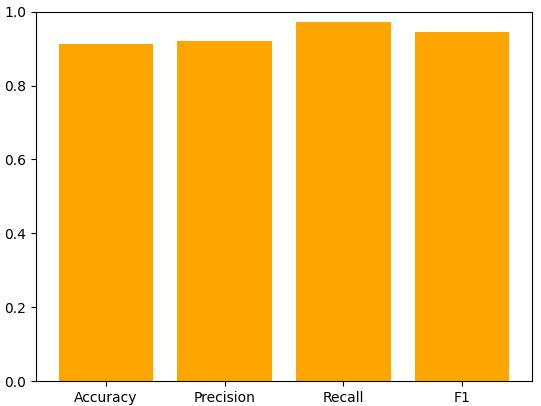
\includegraphics[width=4.6in]{resultados-trafilatura.jpg}
    \caption{Gráfica - Resultados de la evaluación de Trafilatura}
    \label{img:grafica - resultados de la evaluacion de trafilatura}
\end{figure}

\begin{codefloat}
    \inputencoding{latin1}
    \lstinputlisting[style=CppExample, showstringspaces=false]{scripts/script-trafilatura-precision.py}
    \inputencoding{utf8}
    \caption{Función de ejecución de Trafilatura \emph{(precision)}}
    \label{cod:funcion de ejecucion de trafilatura precision}
\end{codefloat}

Veamos las diferentes configuraciones de \textbf{Trafilatura} para potenciar la calidad del texto extraído.
En primer lugar, vamos a mejorar la precisión del algoritmo. Como se puede observar en el fragmento de
código \ref{cod:funcion de ejecucion de trafilatura precision}, se activan además los algoritmos de respaldo.

\begin{table}[h]
    \begin{center}
      \begin{tabular}{| c | c | c | c | c | c | c | c |} \hline 
       \textbf{Nombre} & \textbf{Accuracy} & \textbf{Precision}  & \textbf{Recall} & \textbf{F1} & \textbf{RAM(\%)} & \textbf{CPU(\%)} & \textbf{Time Exec.(s)} \\ \hline
       Tra. precision & 0.9129 & 0.9208 & 0.9699 & 0.9447 & 45.9 & 1.4 & 4.4590 \\ \hline
      \end{tabular}
      \caption{Tabla - Resultados de la evaluación de Trafilatura \emph{precision}}
      \label{tab:tabla - resultados de la evaluacion de trafilatura precision}
    \end{center}
\end{table}

Podemos observar en la tabla \ref{tab:tabla - resultados de la evaluacion de trafilatura precision}, que
los resultados obtenidos reflejan una mínima mejora en lo referido a la \emph{precision}. Algo sorprendente
es que la inclusión de los algoritmos de respaldo no aumentan el uso de recursos ni el tiempo de ejecución.

\begin{figure}[tphb]
    \centering
    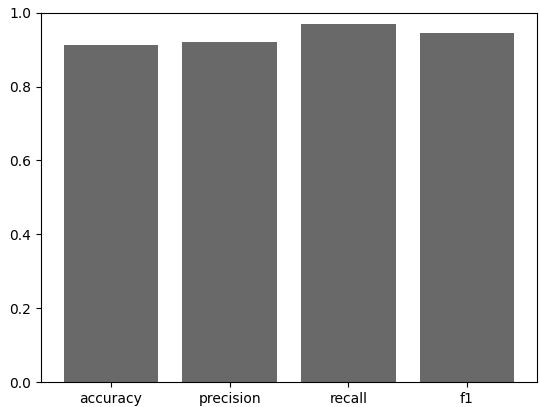
\includegraphics[width=4.5in]{resultados-trafilatura-precision.jpg}
    \caption{Gráfica - Resultados de la evaluación de Trafilatura \emph{precision}}
    \label{img:grafica - resultados de la evaluacion de trafilatura precision}
\end{figure}

\begin{codefloat}
    \inputencoding{latin1}
    \lstinputlisting[style=CppExample, showstringspaces=false]{scripts/script-trafilatura-recall.py}
    \inputencoding{utf8}
    \caption{Función de ejecución de Trafilatura \emph{(recall)}}
    \label{cod:funcion de ejecucion de trafilatura recall}
\end{codefloat}

Otra de las configuraciones permite mejorar la capacidad de captar las partes deseadas del documento, es
decir, permite aumentar el valor de la métrica \emph{recall}. Como podemos observar en el fragmento de
código \ref{cod:funcion de ejecucion de trafilatura recall} los algoritmos de respaldo siguen activos. 
Veamos los resultados obtenidos.

\begin{table}[h]
    \begin{center}
      \begin{tabular}{| c | c | c | c | c | c | c | c |} \hline 
       \textbf{Nombre} & \textbf{Accuracy} & \textbf{Precision}  & \textbf{Recall} & \textbf{F1} & \textbf{RAM(\%)} & \textbf{CPU(\%)} & \textbf{Time Exec.(s)} \\ \hline
       Tra. recall & 0.9188 & 0.9287 & 0.9776 & 0.9525 & 46.3 & 0.5 & 3.0888 \\ \hline
      \end{tabular}
      \caption{Tabla - Resultados de la evaluación de Trafilatura \emph{recall}}
      \label{tab:tabla - resultados de la evaluacion de trafilatura recall}
    \end{center}
\end{table}

\begin{figure}[tphb]
    \centering
    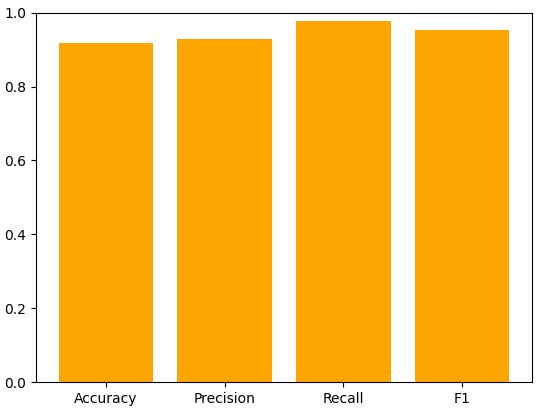
\includegraphics[width=5in]{resultados-trafilatura-recall.jpg}
    \caption{Gráfica - Resultados de la evaluación de Trafilatura \emph{recall}}
    \label{img:grafica - resultados de la evaluacion de trafilatura recall}
\end{figure}

En los resultados mostrados en la tabla \ref{tab:tabla - resultados de la evaluacion de trafilatura recall}
y en la gráfica \ref{img:grafica - resultados de la evaluacion de trafilatura recall}, se puede observar
que nuevamente la mejora es mínima. La calidad de la información extraída es prácticamente la misma que la
ofrecida por la heurística anterior.

Haciendo una comparación más amplia entre los tres tipos de configuraciones para \textbf{Trafilatura},
podemos observar que la heurística dedicada a seleccionar las partes deseadas de un documento es la más
refinada. Esta supera incluso el valor de la métrica \emph{precision} de la propia heurística dedicada a 
ello. Véase \ref{img:grafica - comparacion entre los tres algoritmos de trafilatura}.

\begin{table}[h]
    \begin{center}
      \begin{tabular}{| c | c | c | c | c | c | c | c |} \hline 
       \textbf{Nombre} & \textbf{Accuracy} & \textbf{Precision}  & \textbf{Recall} & \textbf{F1} & \textbf{RAM(\%)} & \textbf{CPU(\%)} & \textbf{Time Exec.(s)} \\ \hline
       Trafilatura & 0.9124 & 0.9196 & 0.9707 & 0.9444 & 45.7 & 1.4 & 4.3919 \\ \hline
       Tra. precision & 0.9129 & 0.9208 & 0.9699 & 0.9447 & 45.9 & 1.4 & 4.4590 \\ \hline
       Tra. recall & 0.9188 & 0.9287 & 0.9776 & 0.9525 & 46.3 & 0.5 & 3.0888 \\ \hline
      \end{tabular}
      \caption{Tabla - Comparación entre los tres algoritmos de Trafilatura}
      \label{tab:tabla - comparacion entre los tres algoritmos de trafilatura}
    \end{center}
\end{table}

Por otra parte, los valores de referidos al uso de recursos del entorno de ejecución también se ven
reducidos en la configuración para \emph{recall}. Al parecer la ejecución de los algoritmos de respaldo no
afecta al consumo de recursos del entorno de ejecución. Véase 
\ref{img:grafica - comparacion entre los tres algoritmos de trafilatura 2}.

\begin{figure}[tphb]
    \centering
    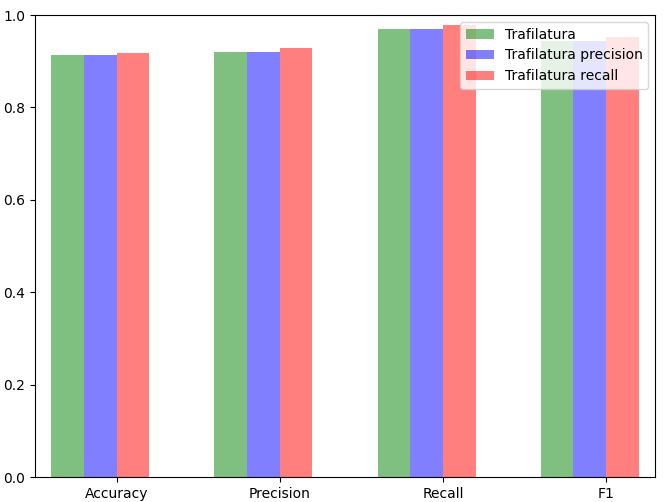
\includegraphics[width=5in]{resultados-trafilatura-comparacion.jpg}
    \caption{Gráfica - Comparación entre los tres algoritmos de Trafilatura}
    \label{img:grafica - comparacion entre los tres algoritmos de trafilatura}
\end{figure}

\begin{figure}[tphb]
    \centering
    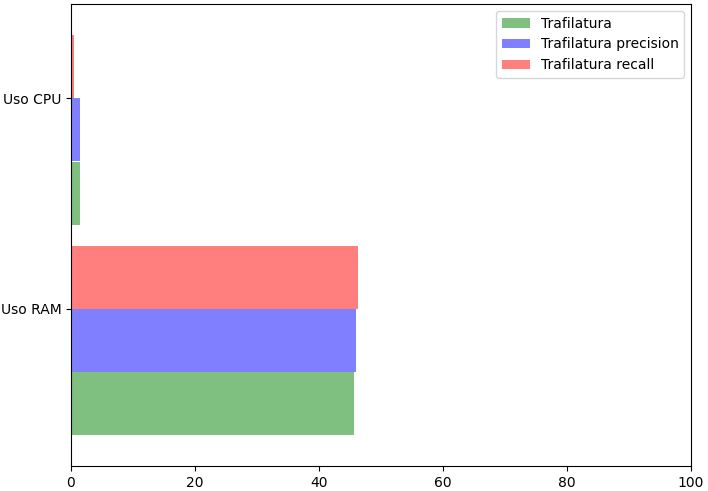
\includegraphics[width=5in]{resultados-trafilatura-comparacion2.jpg}
    \caption{Gráfica - Comparación entre los tres algoritmos de Trafilatura 2}
    \label{img:grafica - comparacion entre los tres algoritmos de trafilatura 2}
\end{figure}

\section*{Goose3}

El siguiente paquete sometido a análisis es \textbf{Goose3}, el cual debemos instalar e importar en el 
fragmento de código respectivo. En cuanto a su instalación, simplemente se debe ejecutar la siguiente 
instrucción en la línea de comandos: \emph{\$ pip install goose3}.

\begin{codefloat}
    \inputencoding{latin1}
    \lstinputlisting[style=CppExample, showstringspaces=false]{scripts/script-goose3.py}
    \inputencoding{utf8}
    \caption{Función de ejecución de Goose3}
    \label{cod:funcion de ejecucion de goose3}
\end{codefloat}

Al igual que otros algoritmos ya vistos, \textbf{Goose3} permite modificar parte de su configuración con el
objetivo de personalizar la salida obtenida. Hay dos formas de pasar la configuración. La primera consiste
en pasarle al algoritmo un objeto \emph{Configuration()}, la segunda es a través de un diccionario de 
configuración.

\begin{Schunk}
    \begin{Soutput}
    >>> g = Goose({'browser_user_agent': 'Mozilla'})
    >>> g = Goose({'browser_user_agent': 'Mozilla', 'parser_class':'soup'})
    ...
    >>> g = Goose({'strict': False})
    \end{Soutput}
\end{Schunk}

En el fragmento de código \ref{cod:funcion de ejecucion de goose3} se muestra las líneas de código empleadas
para que \textbf{Goose3} pueda extraer la información deseada de documentos HTML. Se observa que la forma
de actuar es la misma que en el resto de algoritmos ya vistos. 

\begin{table}[h]
    \begin{center}
      \begin{tabular}{| c | c | c | c | c | c | c | c |} \hline 
       \textbf{Nombre} & \textbf{Accuracy} & \textbf{Precision}  & \textbf{Recall} & \textbf{F1} & \textbf{RAM(\%)} & \textbf{CPU(\%)} & \textbf{Time Exec.(s)} \\ \hline
       Goose3 & 0.8658 & 0.9273 & 0.8913 & 0.9089 & 32.2 & 6.1 & 25.9731 \\ \hline
      \end{tabular}
      \caption{Tabla - Resultados de la evaluación de Goose3}
      \label{tab:tabla - resultados de la evaluacion de goose3}
    \end{center}
\end{table}

En cuanto a calidad de extracción, en la tabla \ref{tab:tabla - resultados de la evaluacion de goose3}
podemos observar que los valores son buenos. La mayor parte del texto extraído son partes deseadas y la 
exclusión de contenido \emph{boilerplate} también es muy buena.

En contrapartida, los valores referentes a la optimización de recursos y tiempo de ejecución, dejan algo
que desear. Además del exagerado tiempo que tarda el algoritmo en ejecutar, el uso de CPU es elevado
respecto a otros algoritmos.

\begin{figure}[tphb]
    \centering
    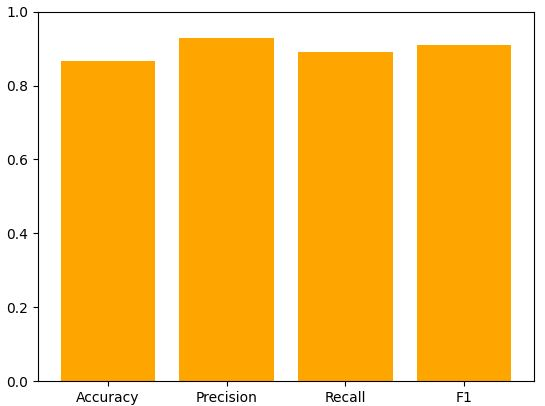
\includegraphics[width=5in]{resultados-goose3.jpg}
    \caption{Gráfica - Resultados de la evaluación de Goose3}
    \label{img:grafica - resultados de la evaluacion de goose3}
\end{figure}

\section*{Boilerpy}

Otro de los paquetes sometidos a análisis es \textbf{Boilerpy}, el cual debemos instalar e importar en el 
fragmento de código respectivo. En cuanto a su instalación, simplemente se debe ejecutar la siguiente 
instrucción en la línea de comandos: \emph{\$ pip install boilerpy3}.

\begin{codefloat}
    \inputencoding{latin1}
    \lstinputlisting[style=CppExample, showstringspaces=false]{scripts/script-boilerpy.py}
    \inputencoding{utf8}
    \caption{Función de ejecución de Boilerpy}
    \label{cod:funcion de ejecucion de boilerpy 2}
\end{codefloat}

En el fragmento de código \ref{cod:funcion de ejecucion de boilerpy 2} se muestra como \textbf{Boilerpy}
extrae texto de diferentes documentos HTML. Recordemos que el algoritmo disponía de múltiples extractores
que se usaban dependiendo del tipo de información a obtener. En este caso se emplea \emph{ArticleExtractor()}
el cual extrae el texto de artículos.

En cuanto a los resultados obtenidos, entran dentro de lo estándar. La calidad del texto que se extrae es
buena y el uso de recursos es reducido. Véase \ref{tab:tabla - resultados de la evaluacion de boilerpy} y 
\ref{img:grafica - resultados de la evaluacion de boilerpy}.

\begin{table}[h]
    \begin{center}
      \begin{tabular}{| c | c | c | c | c | c | c | c |} \hline 
       \textbf{Nombre} & \textbf{Accuracy} & \textbf{Precision}  & \textbf{Recall} & \textbf{F1} & \textbf{RAM(\%)} & \textbf{CPU(\%)} & \textbf{Time Exec.(s)} \\ \hline
       Boilerpy & 0.7947 & 0.8544 & 0.8803 & 0.8672 & 43.9 & 1.9 & 2.5412 \\ \hline
      \end{tabular}
      \caption{Tabla - Resultados de la evaluación de Boilerpy}
      \label{tab:tabla - resultados de la evaluacion de boilerpy}
    \end{center}
\end{table}

\begin{figure}[tphb]
    \centering
    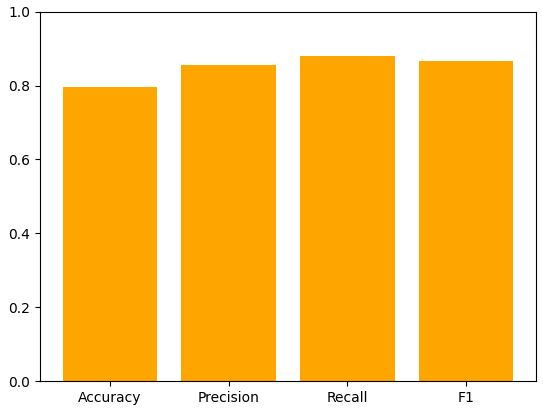
\includegraphics[width=5in]{resultados-boilerpy.jpg}
    \caption{Gráfica - Resultados de la evaluación de Boilerpy}
    \label{img:grafica - resultados de la evaluacion de boilerpy}
\end{figure}

\section*{BoilerpipeR}

La version en \textbf{R} de \textbf{Boilerpy} es \textbf{BoilerpipeR}, el cual debemos instalar e importar 
en el fragmento de código respectivo. En cuanto a su instalación, simplemente se debe ejecutar la siguiente 
instrucción en la línea de comandos de R: \emph{install.packages("boilerpipeR")}.

\begin{codefloat}
    \inputencoding{latin1}
    \lstinputlisting[style=CppExample, showstringspaces=false]{scripts/script-boilerpiper.py}
    \inputencoding{utf8}
    \caption{Ejecución de BoilerpipeR desde Python}
    \label{cod:ejecucion de boilerpiper desde python}
\end{codefloat}

Al ser este un paquete propio de R, es necesaria una interfaz que nos permita ejecutarlo en Python. En el
fragmento de código \ref{cod:ejecucion de boilerpiper desde python} se muestra el proceso.

Por otro lado, en cuanto a la propia función de ejecución, se puede observar en el fragmento de código
\ref{cod:funcion de ejecucion de boilerpiper 2} como está programado el algoritmo. Podemos observar que la 
forma de proceder es similar a la ya propuesta por los algoritmos de otras herramientas de minado.

\begin{codefloat}
    \inputencoding{latin1}
    \lstinputlisting[style=CppExample, showstringspaces=false]{scripts/script-boilerpiper.R}
    \inputencoding{utf8}
    \caption{Función de ejecución de BoilerpipeR}
    \label{cod:funcion de ejecucion de boilerpiper 2}
\end{codefloat}

\begin{table}[h]
    \begin{center}
      \begin{tabular}{| c | c | c | c | c | c | c | c |} \hline 
       \textbf{Nombre} & \textbf{Accuracy} & \textbf{Precision}  & \textbf{Recall} & \textbf{F1} & \textbf{RAM(\%)} & \textbf{CPU(\%)} & \textbf{Time Exec.(s)} \\ \hline
       BoilerpipeR & 0.7830 & 0.8486 & 0.8696 & 0.8590 & 47.9 & 2.6 & 39.9543 \\ \hline
      \end{tabular}
      \caption{Tabla - Resultados de la evaluación de BoilerpipeR}
      \label{tab:tabla - resultados de la evaluacion de boilerpiper}
    \end{center}
\end{table}

Realizando una apreciación general sobre los datos obtenidos, podemos observar que \textbf{BoilerpipeR}
realiza un buen trabajo de minado, véase \ref{tab:tabla - resultados de la evaluacion de boilerpiper}.
Comparemos ahora los resultados obtenidos, con los calculados anteriormente para \textbf{Boilerpy}.

\begin{table}[h]
    \begin{center}
      \begin{tabular}{| c | c | c | c | c | c | c | c |} \hline 
       \textbf{Nombre} & \textbf{Accuracy} & \textbf{Precision}  & \textbf{Recall} & \textbf{F1} & \textbf{RAM(\%)} & \textbf{CPU(\%)} & \textbf{Time Exec.(s)} \\ \hline
       Boilerpy & 0.7947 & 0.8544 & 0.8803 & 0.8672 & 43.9 & 1.9 & 2.5412 \\ \hline
       BoilerpipeR & 0.7830 & 0.8486 & 0.8696 & 0.8590 & 47.9 & 2.6 & 39.9543 \\ \hline
      \end{tabular}
      \caption{Tabla - Comparación de resultados entre Boilerpy \& BoilerpipeR}
      \label{tab:tabla - comparacion de resultados entre boilerpy y boilerpiper}
    \end{center}
\end{table}

Se muestra en la tabla \ref{tab:tabla - comparacion de resultados entre boilerpy y boilerpiper} los datos
obtenidos para ambas herramientas. En ambos algoritmos se ha empleado \emph{ArticleExtractor} como extractor
estándar. Podemos observar que apenas existen claras diferencias entre ambos resultados, respecto a la
calidad del texto extraído, las dos herramientas reflejan unos resultados muy parejos.

En contrapartida, los resultados obtenidos con respecto a empleo de recursos del entorno de ejecución son
algo diferentes. El tiempo que tarda en ejecutarse \textbf{BoilerpipeR} se aleja demasiado de la media de
algoritmos visto hasta ahora. Veamos una comparación gráfica.

\begin{figure}[tphb]
    \centering
    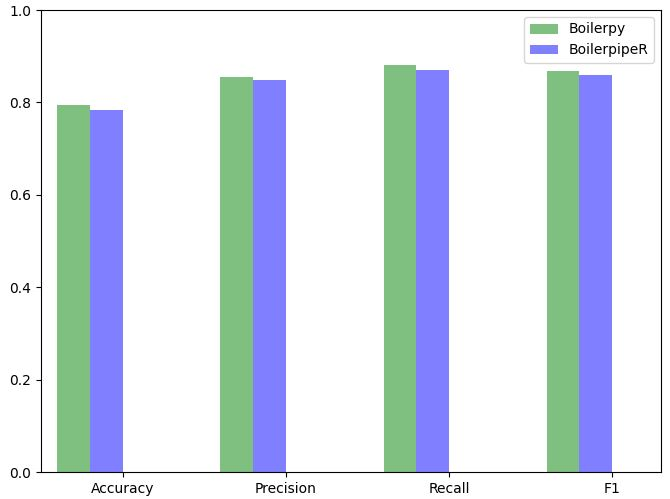
\includegraphics[width=5in]{resultados-boilerpiper.jpg}
    \caption{Gráfica - Resultados de la evaluación de BoilerpipeR}
    \label{img:grafica - resultados de la evaluacion de boilerpiper}
\end{figure}

\begin{figure}[tphb]
    \centering
    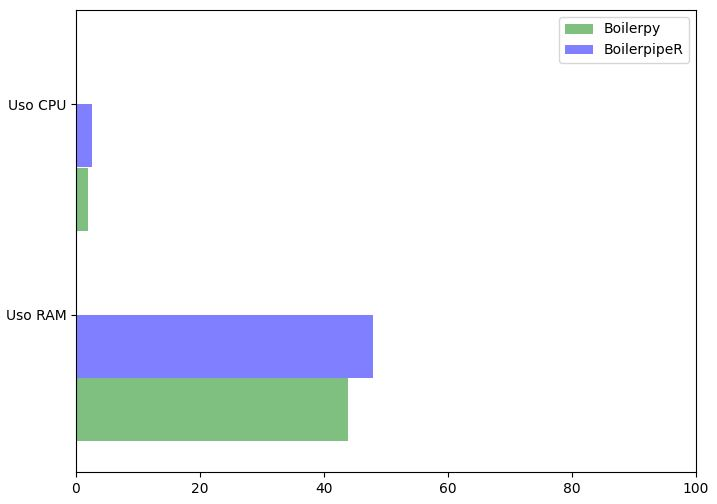
\includegraphics[width=5in]{resultados-boilerpiper2.jpg}
    \caption{Gráfica - Resultados de la evaluación de BoilerpipeR 2}
    \label{img:grafica - resultados de la evaluacion de boilerpiper 2}
\end{figure}

\section*{rvest}

El siguiente paquete sometido a análisis es \textbf{rvest}, el cual debemos instalar e importar en el
fragmento de código respectivo. En cuanto a su instalación, simplemente se debe ejecutar la siguiente
instrucción en la línea de comandos de R: \emph{install.packages("rvest")}.

\begin{codefloat}
    \inputencoding{latin1}
    \lstinputlisting[style=CppExample, showstringspaces=false]{scripts/script-rvest.py}
    \inputencoding{utf8}
    \caption{Ejecución de rvest desde Python}
    \label{cod:ejecucion de rvest desde python}
\end{codefloat}

\begin{codefloat}
    \inputencoding{latin1}
    \lstinputlisting[style=CppExample, showstringspaces=false]{scripts/script-rvest.R}
    \inputencoding{utf8}
    \caption{Función de ejecución de rvest}
    \label{cod:funcion de ejecucion de rvest}
\end{codefloat}

En el fragmento de código \ref{cod:funcion de ejecucion de rvest} se muestra la función empleada para
ejecutar \textbf{rvest}. Se puede observar el empleo del operador tubería \emph{\%>\%} el cual se encarga
de facilitar la transferencia de resultados de las diferentes funciones implicadas.

\begin{table}[h]
    \begin{center}
      \begin{tabular}{| c | c | c | c | c | c | c | c |} \hline 
       \textbf{Nombre} & \textbf{Accuracy} & \textbf{Precision}  & \textbf{Recall} & \textbf{F1} & \textbf{RAM(\%)} & \textbf{CPU(\%)} & \textbf{Time Exec.(s)} \\ \hline
       rvest & 0.1347 & 0.1371 & 0.8974 & 0.2378 & 44.1 & 8.9 & 60.3245 \\ \hline
      \end{tabular}
      \caption{Tabla - Resultados de la evaluación de rvest}
      \label{tab:tabla - resultados de la evaluacion de rvest}
    \end{center}
\end{table}

En cuanto a las métricas, los datos reflejados en \ref{tab:tabla - resultados de la evaluacion de rvest}
dejan bastante claro que la calidad de \textbf{rvest} en la extracción de contenido no es buena. Uno de
los principales motivos es el uso necesario de expresiones \emph{xPath}. En este caso \emph{xpath = //body} 
permite al algoritmo trabajar con la etiqueta \emph{body} del documento HTML en cuestión.

\begin{figure}[tphb]
    \centering
    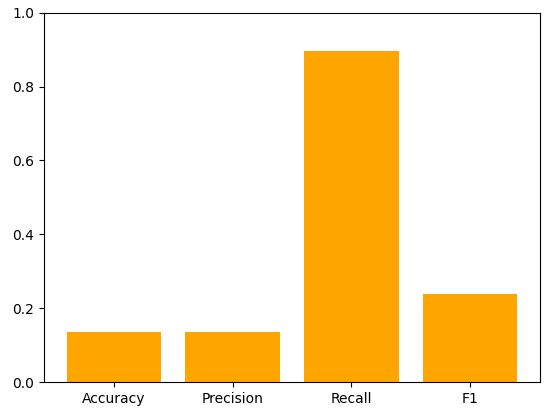
\includegraphics[width=5in]{resultados-rvest.jpg}
    \caption{Gráfica - Resultados de la evaluación de rvest}
    \label{img:grafica - resultados de la evaluacion de rvest}
\end{figure}

\section*{Rcrawler}

Otro paquete propio de R sometido a análisis será \textbf{Rcrawler}, el cual debemos instalar e importar
en el fragmento de código respectivo. En cuanto a su instalación, simplemente se debe ejecutar la siguiente
instrucción en la línea de comandos: \emph{install.packages("Rcrawler", dependencies = TRUE)}.

\begin{codefloat}
    \inputencoding{latin1}
    \lstinputlisting[style=CppExample, showstringspaces=false]{scripts/script-rcrawler.R}
    \inputencoding{utf8}
    \caption{Función de ejecución de Rcrawler}
    \label{cod:funcion de ejecucion de rcrawler}
\end{codefloat}

En referencia al fragmento de código mostrado en \ref{cod:funcion de ejecucion de rcrawler}, es muy similar
al resto de códigos ya mostrados anteriormente. En este caso se deben emplear nuevamente expresiones
\emph{xPath} para trabajar sobre la etiqueta HTML requerida, \emph{XpathPatterns = "//body"}.

\begin{codefloat}
    \inputencoding{latin1}
    \lstinputlisting[style=CppExample, showstringspaces=false]{scripts/script-rcrawler.py}
    \inputencoding{utf8}
    \caption{Ejecución de Rcrawler desde Python}
    \label{cod:ejecucion de rcrawler desde python}
\end{codefloat}

Sobre los datos obtenidos, se muestran en la tabla \ref{tab:tabla - resultados de la evaluacion de rcrawler}.
Estos reflejan una pobre calidad de la información extraída por parte de \textbf{Rcrawler}. Al igual que
sucedía con \textbf{rvest}, el empleo de expresiones \emph{xPath} limita la información a extraer. Por otro 
lado, ni el empleo de recursos, ni el tiempo de ejecución son buenos.

\begin{table}[h]
    \begin{center}
      \begin{tabular}{| c | c | c | c | c | c | c | c |} \hline 
       \textbf{Nombre} & \textbf{Accuracy} & \textbf{Precision}  & \textbf{Recall} & \textbf{F1} & \textbf{RAM(\%)} & \textbf{CPU(\%)} & \textbf{Time Exec.(s)} \\ \hline
       Rcrawler & 0.4540 & 0.4628 & 0.9310 & 0.6181 & 46.7 & 3.4 & 158.0663 \\ \hline
      \end{tabular}
      \caption{Tabla - Resultados de la evaluación de Rcrawler}
      \label{tab:tabla - resultados de la evaluacion de rcrawler}
    \end{center}
\end{table}

\begin{figure}[tphb]
    \centering
    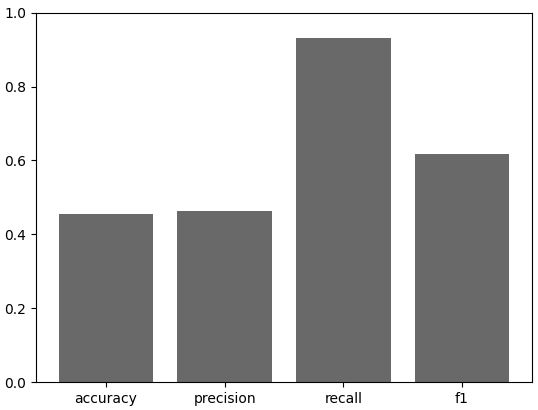
\includegraphics[width=5in]{resultados-rcrawler.jpg}
    \caption{Gráfica - Resultados de la evaluación de Rcrawler}
    \label{img:grafica - resultados de la evaluacion de rcrawler}
\end{figure}

\section*{htm2txt}

Veamos como funciona el paquete \textbf{htm2txt}, para ello primero debemos realizar la instalación e
importación en el fragmento de código respectivo. En cuanto a su instalación, simplemente se debe ejecutar
la siguiente instrucción en la línea de comandos de R: \emph{install.packages('htm2txt')}.

\begin{codefloat}
    \inputencoding{latin1}
    \lstinputlisting[style=CppExample, showstringspaces=false]{scripts/script-htm2txt.R}
    \inputencoding{utf8}
    \caption{Función de ejecución de htm2txt}
    \label{cod:funcion de ejecucion de htm2txt}
\end{codefloat}

\begin{codefloat}
    \inputencoding{latin1}
    \lstinputlisting[style=CppExample, showstringspaces=false]{scripts/script-htm2txt.py}
    \inputencoding{utf8}
    \caption{Ejecución de htm2txt desde Python}
    \label{cod:ejecucion de htm2txt desde python}
\end{codefloat}

En cuanto al fragmento de código mostrado en \ref{cod:funcion de ejecucion de htm2txt}, es muy similar al
resto de códigos ya vistos anteriormente. En este caso no entran en juego expresiones \emph{xPath}, sino
que es directamente la propia heurística del algoritmo la que se encarga de seleccionar el contenido válido.

Si recordamos la heurística de \textbf{htm2txt}, esta se encargaba de utilizar expresiones regulares para
eliminar las etiquetas de los documentos HTML pertinentes. En esta heurística tan simple, funciones como 
\emph{gsub()} tomaban mucha relevancia.

\begin{table}[h]
    \begin{center}
      \begin{tabular}{| c | c | c | c | c | c | c | c |} \hline 
       \textbf{Nombre} & \textbf{Accuracy} & \textbf{Precision}  & \textbf{Recall} & \textbf{F1} & \textbf{RAM(\%)} & \textbf{CPU(\%)} & \textbf{Time Exec.(s)} \\ \hline
       htm2txt & 0.4547 & 0.4714 & 0.8885 & 0.6160 & 46.7 & 2.0 & 80.5288 \\ \hline
      \end{tabular}
      \caption{Tabla - Resultados de la evaluación de htm2txt}
      \label{tab:tabla - resultados de la evaluacion de htm2txt}
    \end{center}
\end{table}

Los resultados mostrados en la tabla \ref{tab:tabla - resultados de la evaluacion de htm2txt} reflejan la
simplicidad del algoritmo. El uso único de expresiones regulares hace que la calidad del texto extraído
no sea buena. Por otro lado, el tiempo de ejecución es demasiado alto.

\begin{figure}[tphb]
    \centering
    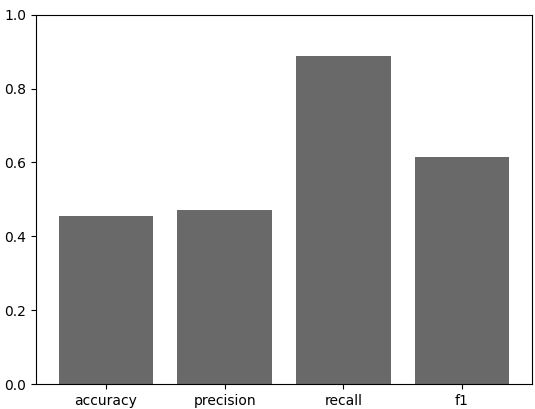
\includegraphics[width=5in]{resultados-htm2txt.jpg}
    \caption{Gráfica - Resultados de la evaluación de htm2txt}
    \label{img:grafica - resultados de la evaluacion de htm2txt}
\end{figure}

\section*{Expresiones xPath}

¿Qué ocurre si solo empleamos expresiones \emph{xPath} sin ningún tipo de heurística? Lo obvio seria que
los resultados obtenidos fuesen peores de los ya calculados. Por otro lado, para analizar el documento se 
usara \emph{lxml}, veamos.

\begin{codefloat}
    \inputencoding{latin1}
    \lstinputlisting[style=CppExample, showstringspaces=false]{scripts/script-xpath.py}
    \inputencoding{utf8}
    \caption{Función de ejecución de \emph{xPath}}
    \label{cod:funcion de ejecucion de xpath}
\end{codefloat}

En cuanto al fragmento de código \ref{cod:funcion de ejecucion de xpath}, lo único a destacar es la expresión
\emph{xPath} usada. Para cada artículo queremos obtener el cuerpo del mismo, por ello se accede a la 
etiqueta \emph{body} del mismo. Por otro lado, para refinar la solución obtenida, eliminamos las expresiones 
propias de la estructuración del texto.

\begin{table}[h]
    \begin{center}
      \begin{tabular}{| c | c | c | c | c | c | c | c |} \hline 
       \textbf{Nombre} & \textbf{Accuracy} & \textbf{Precision}  & \textbf{Recall} & \textbf{F1} & \textbf{RAM(\%)} & \textbf{CPU(\%)} & \textbf{Time Exec.(s)} \\ \hline
       xPath & 0.2421 & 0.2401 & 0.9915 & 0.3866 & 44.4 & 2.0 & 0.7476 \\ \hline
      \end{tabular}
      \caption{Tabla - Resultados de la evaluación de \emph{xPath}}
      \label{tab:tabla - resultados de la evaluacion de xpath}
    \end{center}
\end{table}

Si observamos la tabla \ref{tab:tabla - resultados de la evaluacion de xpath} podemos comprobar que los
resultados obtenidos reflejan unas métricas muy pobres. La calidad del texto extraído es muy inferior a la
media del resto de algoritmos. Por otro lado, como era de esperar, el tiempo de ejecución es muy bajo, pues
al no disponer de heurística propia la cantidad de ejecuciones a realizar es menor.

\begin{figure}[tphb]
    \centering
    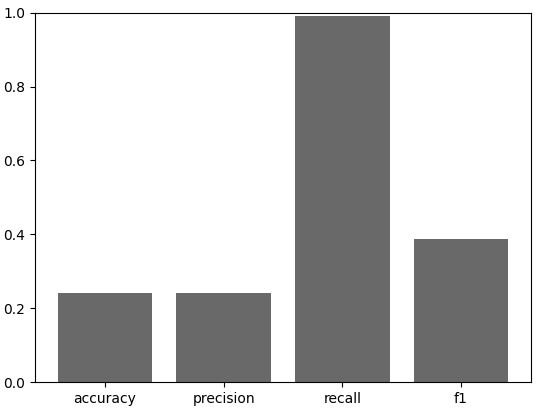
\includegraphics[width=5in]{resultados-xpath.jpg}
    \caption{Gráfica - Resultados de la evaluación de \emph{xPath}}
    \label{img:grafica - resultados de la evaluacion de xpath}
\end{figure}

Este tipo de paquetes o algoritmos que emplean expresiones \emph{xPath}, ya sea como parte de su heurística,
o como única fuente de obtención de información, se emplean mayoritariamente para obtener partes reducidas
de un documento HTML.

\section{Comparación de paquetes}
\label{sec:comparacion de paquetes}

Una vez vistos los resultados individuales de cada paquete, veamos una comparación de los mismos desde
diferentes puntos de vista. El objetivo de esta comparación es obtener de una manera más clara cuáles son
los causantes de los diferentes resultados obtenidos. En muchos casos, el analizador empleado, la heurística,
o el propio lenguaje de programación se convierten en un factor fundamental.

\subsection{Comparación de paquetes que usan expresiones \emph{xPath}}
\label{subsec:comparacion de paquetes que usan expresiones xpath}

El uso de expresiones regulares es una técnica conocida que puede utilizarse en el proceso de extracción,
se determina un cierto patrón y se buscan etiquetas a lo largo del documento que coincidan. Sin embargo,
pueden existir problemas cuando el número de etiquetas internas es ambiguo \cite{uzun}. Para una regla de 
extracción, existen dos técnicas. Se puede buscar en el documento todos los registros encontrados de la 
expresión regular, o el proceso de extracción puede finalizar con la búsqueda del primer registro \cite{regex}.

En este caso, la comparación abordará aquellos paquetes que basen su heurística a partir del uso de este
tipo de expresiones. Paquetes como \emph{Rcrawler} y \emph{rvest} serán los seleccionados, entre otros.
Cabe mencionar que la comparación se realizará a partir de las métricas calculadas en la sección anterior.
Además, será interesante ver una comparación con el simple empleo de expresiones \emph{xPath}.

\begin{table}[h]
    \begin{center}
      \begin{tabular}{| c | c | c | c | c | c | c | c |} \hline 
       \textbf{Nombre} & \textbf{Accuracy} & \textbf{Precision}  & \textbf{Recall} & \textbf{F1} & \textbf{RAM(\%)} & \textbf{CPU(\%)} & \textbf{Time Exec.(s)} \\ \hline
       rvest & 0.1347 & 0.1371 & 0.8974 & 0.2378 & 44.1 & 8.9 & 60.3245 \\ \hline
       Rcrawler & 0.4540 & 0.4628 & 0.9310 & 0.6181 & 46.7 & 3.4 & 158.0663 \\ \hline
       xPath & 0.2421 & 0.2401 & 0.9915 & 0.3866 & 44.4 & 2.0 & 0.7476 \\ \hline
      \end{tabular}
      \caption{Tabla - Comparación de paquetes que usan expresiones \emph{xPath}}
      \label{tab:tabla - comparacion de paquetes que usan expresiones xpath}
    \end{center}
\end{table}

Podemos observar en la tabla \ref{tab:tabla - comparacion de paquetes que usan expresiones xpath} los
resultados obtenidos por los paquetes que emplean expresiones \emph{xPath}. De manera general podemos decir
que los resultados dejan bastante que desear. Resultados muy pobres para el tiempo de ejecución empleado.
Veamos ahora una comparación más minuciosa, observando las diferencias entre las métricas de forma individual.

\begin{figure}[tphb]
    \centering
    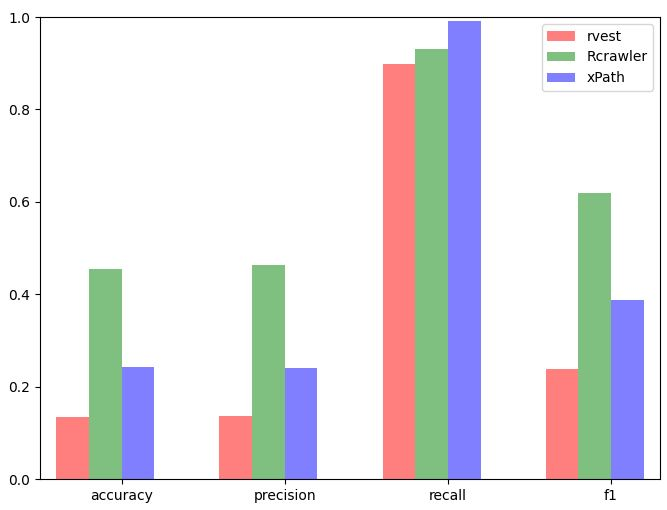
\includegraphics[width=5.3in]{resultados-comparacion-xpath.jpg}
    \caption{Gráfica - Comparación de paquetes que usan expresiones \emph{xPath}}
    \label{img:grafica - comparacion de paquetes que usan expresiones xpath}
\end{figure}

En la gráfica \ref{img:grafica - comparacion de paquetes que usan expresiones xpath} podemos observar de 
manera más visual los resultados obtenidos. Sorprende que \textbf{rvest} tenga unos resultados tan pobres, 
siendo superado incluso por expresiones regulares. Por otro lado, \textbf{Rcrawler} sin tener resultados 
buenos, es el único que realiza un decente proceso de \emph{web scraping}.

¿Cómo es posible que se haya captado la mayor parte del contenido principal y los resultados del resto de
métricas sean tan malos? La razón es que además de captar contenido principal, el algoritmo ha captado
contenido no deseado, esto empeora la calidad de la solución. Si observamos la relación entre la variable
\emph{recall} y la variable \emph{precision}, nos damos cuenta de que captación de contenido principal es
buena, pero la exclusión de contenido \emph{boilerplate} no lo es tanto.

\begin{figure}[tphb]
    \centering
    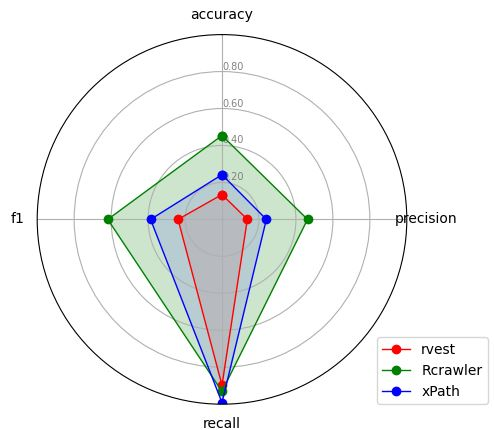
\includegraphics[width=5.3in]{eficacia-general-xpath.jpg}
    \caption{Comparación de la eficacia en los paquetes que usan expresiones \emph{xPath}}
    \label{img:comparacion de la eficacia en los paquetes que usan expresiones xPath}
\end{figure}

Vistos los diferentes resultados obtenidos, y observando la imagen 
\ref{img:comparacion de la eficacia en los paquetes que usan expresiones xPath} podemos concluir que los 
algoritmos sometidos a evaluación que emplean expresiones \emph{xPath} no realizan un minado web de calidad. 
Por otro lado, los resultados referentes al rendimiento y optimización de los mismos tampoco son buenos.

Si estos algoritmos no ofrecen un resultado de calidad y su rendimiento no es bueno, ¿por qué son tan
utilizados? La respuesta es que este tipo de algoritmos son buenos cuando deseas encontrar determinadas
etiquetas dentro de un documento HTML y la calidad de la solución no es importante. Imaginemos que se desea
conocer el precio de un determinado producto en diferentes páginas web. Puesto que dicho precio estará
dentro de una cierta etiqueta HTML, el empleo de una heurística compleja no tendría mucho sentido, además
de que reduciría tiempos de ejecución.

\subsection{Comparación de paquetes según el analizador empleado}
\label{subsec:comparacion de paquetes segun el analizador empleado}

El uso de expresiones regulares es una técnica conocida que puede utilizarse en el proceso de extracción.
Sin embargo, puede causar problemas cuando el número de etiquetas internas es ambiguo. En esta situación
el empleo de analizadores pueden usarse como una posible solución.

A lo largo del apéndice \ref{cha:analizadores empleados en los paquetes de web scraping}, ya se realizó una 
breve introducción de los analizadores empleados en los algoritmos de \emph{web scraping}. Veamos ahora la
importancia de cada uno en la eficacia de los mismos.

\begin{table}[h]
    \begin{center}
      \begin{tabular}{| c | c | c | c | c | c | c | c |} \hline 
       \textbf{Nombre} & \textbf{Accuracy} & \textbf{Precision}  & \textbf{Recall} & \textbf{F1} & \textbf{RAM(\%)} & \textbf{CPU(\%)} & \textbf{Time Exec.(s)} \\ \hline
       Boilerpy & 0.7947 & 0.8544 & 0.8803 & 0.8672 & 43.9 & 1.9 & 2.5412 \\ \hline
       Goose3 & 0.8658 & 0.9273 & 0.8913 & 0.9089 & 32.2 & 6.1 & 25.9731 \\ \hline
       html2text & 0.5105 & 0.5107 & 0.9804 & 0.6715 & 44.6 & 1.8 & 4.4020 \\ \hline
       Beau. Soup & 0.5165 & 0.5129 & 0.9928 & 0.6764 & 47.0 & 4.3 & 4.0882 \\ \hline
      \end{tabular}
      \caption{Tabla - Paquetes que emplean \emph{html.parser} como analizador}
      \label{tab:tabla - paquetes que emplean html.parser como analizador}
    \end{center}
\end{table}

Empecemos primero con aquellos algoritmos de que emplean \emph{html.parse} como parte de su heurística.
Podemos observar en la tabla \ref{tab:tabla - paquetes que emplean html.parser como analizador} los
resultados obtenidos para los cuatro diferentes algoritmos. Si recordamos como funcionaba \emph{html.parse},
trabaja con etiquetas, además no es un algoritmo excesivamente rápido y es indulgente en su análisis.

\begin{figure}[tphb]
    \centering
    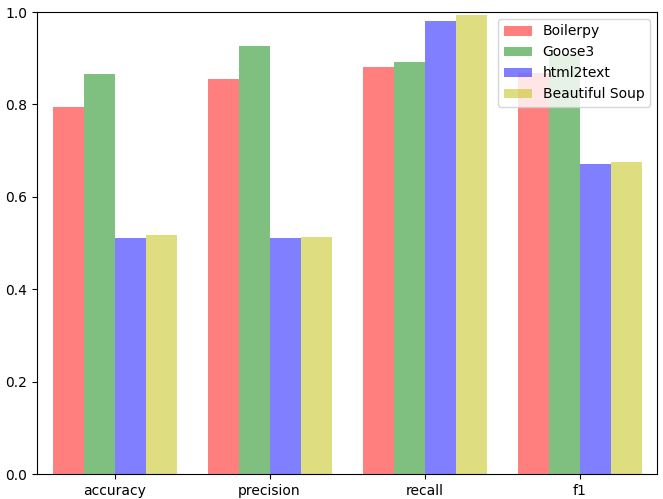
\includegraphics[width=5.5in]{resultados-comparacion-htmlparse.jpg}
    \caption{Gráfica - Comparación de paquetes que usan \emph{html.parser} como analizador}
    \label{img:grafica - comparacion de paquetes que usan html.parser como analizador}
\end{figure}

Si observamos la gráfica \ref{img:grafica - comparacion de paquetes que usan html.parser como analizador},
y ponemos atención en las variables \emph{accuracy} y \emph{precision}, nos damos cuenta de que los valores
mostrados son muy dispares. Al tratar con un analizador tan permisivo, es necesario crear una heurística
elaborada para excluir la mayor cantidad de contenido \emph{boilerplate}.

Siguiendo este aspecto, en cuanto a la captación de contenido principal, todos los algoritmos retornan
buenos resultados. Sorprende incluso ver que los datos mostrados para \textbf{Beautiful Soup} y 
\textbf{html2txt}. Entonces, ¿a qué pueden deberse estas diferencias en las métricas? La explicación es
que \textbf{Boilerpy} y \textbf{Goose3} presentan una heurística más compleja y elaborada.

En cuanto a las métricas dependientes del entorno de ejecución, los valores relativos al uso de memoria
RAM, CPU y tiempo de ejecución empleado son bastante estándar. El único paquete que presenta valores que
difieren del resto es \textbf{Goose3}.

Acabamos de ver el rendimiento de aquellos paquetes que emplean \emph{html.parse} como analizador. Veamos
ahora como se comportan los paquetes que usan \emph{lxml} como parte de su heurística. Podemos observar en 
la tabla \ref{tab:tabla - paquetes que emplean lxml como analizador} los resultados obtenidos para los 
cuatro diferentes algoritmos.

\begin{table}[h]
    \begin{center}
      \begin{tabular}{| c | c | c | c | c | c | c | c |} \hline 
       \textbf{Nombre} & \textbf{Accuracy} & \textbf{Precision}  & \textbf{Recall} & \textbf{F1} & \textbf{RAM(\%)} & \textbf{CPU(\%)} & \textbf{Time Exec.(s)} \\ \hline
       inscriptis & 0.5414 & 0.5404 & 0.9875 & 0.6985 & 45.0 & 0.2 & 2.1009 \\ \hline
       Beau. Soup & 0.5165 & 0.5129 & 0.9928 & 0.6764 & 42.0 & 1.2 & 3.1778 \\ \hline
       html\_text & 0.5166 & 0.5130 & 0.9928 & 0.6765 & 44.9 & 0.5 & 1.1800 \\ \hline
       jusText & 0.7668 & 0.8649 & 0.8573 & 0.8610 & 45.1 & 0.5 & 2.9546 \\ \hline
       readability & 0.8880 & 0.9101 & 0.9370 & 0.9233 & 45.3 & 1.6 & 3.5952 \\ \hline
       trafilatura & 0.9124 & 0.9196 & 0.9928 & 0.9444 & 45.7 & 1.4 & 4.3919 \\ \hline
      \end{tabular}
      \caption{Tabla - Paquetes que emplean \emph{lxml} como analizador}
      \label{tab:tabla - paquetes que emplean lxml como analizador}
    \end{center}
\end{table}

Recordemos que para analizar los diferentes documentos, \emph{lxml} convertía el texto de entrada en una 
estructura de tipo árbol. Esto le permite navegar y encontrar la información requerida de forma más sencilla.
Al igual que \emph{html.parse}, este es un analizador permisivo, por lo que el trabajo de eliminación de 
contenido \emph{boilerplate} será delegado a la heurística determinada.

En cuanto a la comparación de algoritmos, si observamos las variables de \emph{accuracy} y \emph{precision}
en la gráfica \ref{img:grafica - comparacion de paquetes que usan lxml como analizador}, nos damos cuenta
de la disparidad de resultados entre los algoritmos. Mientras que algoritmos como \textbf{inscriptis},
\textbf{Beautiful Soup} o \textbf{html\_text} presentan unos resultados mediocres, el resto se acercan un 
poco más a lo que un usuario final pretendería obtener.

\begin{figure}[tphb]
    \centering
    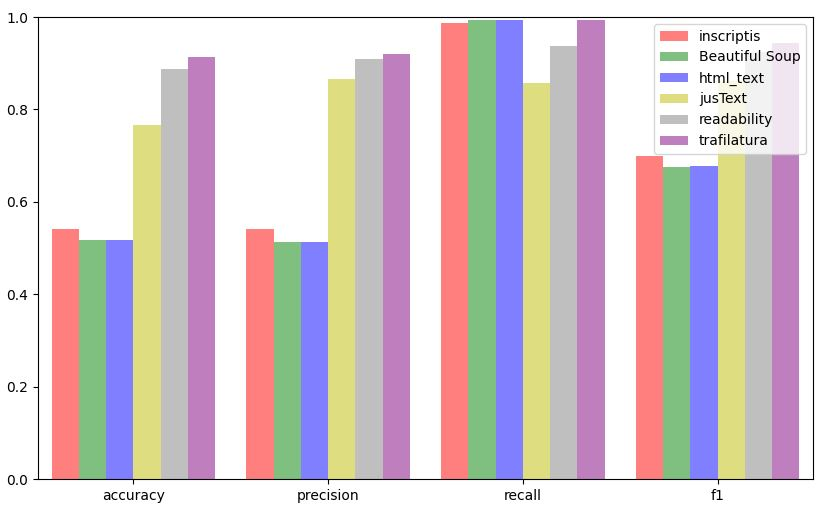
\includegraphics[width=6.5in]{resultados-comparacion-lxml.jpg}
    \caption{Gráfica - Comparación de paquetes que usan \emph{lxml} como analizador}
    \label{img:grafica - comparacion de paquetes que usan lxml como analizador}
\end{figure}

La complejidad de cada algoritmo, también, se ve reflejada en el uso de recursos del medio de ejecución.
Los dos algoritmos más complejos, computacionalmente, son los que más uso hacen de la CPU y que más tardan
en obtener el resultado final.

Veamos por último aquellos paquetes que emplean \emph{XML} o \emph{xml2} como analizador. Ambas librerías
emplean la jerarquía de clases para realizar un análisis. La principal diferencia entre los dos tiene que
ver con la gestión de memoria.

Obsérvese la tabla \ref{tab:tabla - paquetes que emplean xml o xml2 como analizador}, donde se aprecia la
inmensa diferencia entre los tres paquetes. Mientras que \textbf{rvest} y \textbf{Rcrawler} presentan datos
muy pobres, \textbf{boilerpipeR} retorna buenas métricas. Debemos mencionar también la multiplicidad de
extractores que este último presenta, parte de su objetivo es el análisis de este tipo de documentos.

\begin{table}[h]
    \begin{center}
      \begin{tabular}{| c | c | c | c | c | c | c | c |} \hline 
       \textbf{Nombre} & \textbf{Accuracy} & \textbf{Precision}  & \textbf{Recall} & \textbf{F1} & \textbf{RAM(\%)} & \textbf{CPU(\%)} & \textbf{Time Exec.(s)} \\ \hline
       rvest & 0.1347 & 0.1371 & 0.8974 & 0.2378 & 44.1 & 8.9 & 60.3245 \\ \hline
       Rcrawler & 0.4540 & 0.4628 & 0.9310 & 0.6181 & 46.7 & 3.4 & 158.0663 \\ \hline
       boilerpipeR & 0.7830 & 0.8486 & 0.8696 & 0.8590 & 47.9 & 2.6 & 39.9543 \\ \hline
      \end{tabular}
      \caption{Tabla - Paquetes que emplean \emph{XML} o \emph{xml2} como analizador}
      \label{tab:tabla - paquetes que emplean xml o xml2 como analizador}
    \end{center}
\end{table}

Aun recopilando menos cantidad de contenido principal que \textbf{rvest} o \textbf{Rcrawler}, 
\textbf{boilerpipeR} es capaz de obtener la información requerida de forma precisa. De hecho, la efectividad 
del algoritmo es asombrosa, solo hace falta ver la poca diferencia entre puntuación entre \emph{recall} 
con el resto de métricas.

\begin{figure}[tphb]
    \centering
    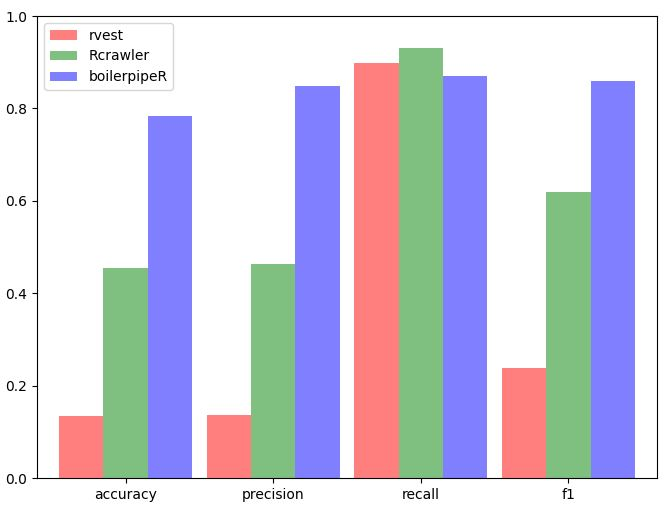
\includegraphics[width=5.5in]{resultados-comparacion-xml-xml2.jpg}
    \caption{Gráfica - Comparación de paquetes que usan \emph{XML} o \emph{xml2} como analizador}
    \label{img:grafica - comparacion de paquetes que usan xml o xml2 como analizador}
\end{figure}

En cuanto al uso de recursos \emph{boilerpipeR} también muestra un uso más óptimo de los mismos. Aunque el
tiempo de ejecución sigue siendo alto para lo que se pretende, es mucho menor que el de \textbf{rvest} o
\textbf{Rcrawler}.


 